\centering
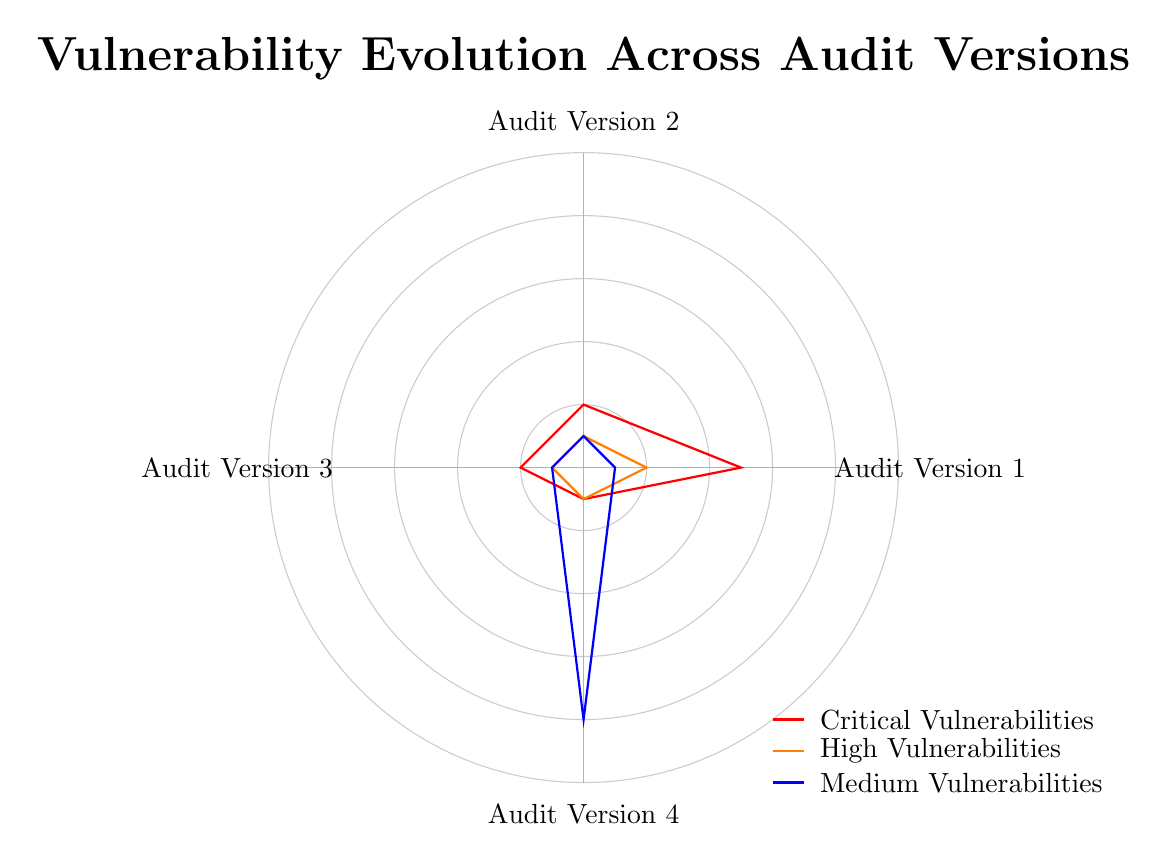
\begin{tikzpicture}[scale=0.4]

% =========================
% CÍRCULOS DE REFERENCIA
% =========================
\foreach \r in {2,4,6,8,10} {
    \draw[gray!40] (0,0) circle (\r);
}

% =========================
% EJES RADIALES + ETIQUETAS
% =========================
\foreach \a/\label in {
    0/{Audit Version 1},
    90/{Audit Version 2},
    180/{Audit Version 3},
    270/{Audit Version 4}
}{
    \draw[gray!60] (0,0) -- (\a:10);
    \node at (\a:11) {\label};
}

% =========================
% SERIE: CRITICAL
% =========================
\draw[red, thick]
    (0:5) --
    (90:2) --
    (180:2) --
    (270:1) --
    cycle;

% =========================
% SERIE: HIGH
% =========================
\draw[orange, thick]
    (0:2) --
    (90:1) --
    (180:1) --
    (270:1) --
    cycle;

% =========================
% SERIE: MEDIUM
% =========================
\draw[blue, thick]
    (0:1) --
    (90:1) --
    (180:1) --
    (270:8) --
    cycle;

% =========================
% LEYENDA
% =========================
\begin{scope}[shift={(6,-8)}]
    \draw[red, thick] (0,0) -- (1,0);
    \node[right] at (1.2,0) {Critical Vulnerabilities};

    \draw[orange, thick] (0,-1) -- (1,-1);
    \node[right] at (1.2,-1) {High Vulnerabilities};

    \draw[blue, thick] (0,-2) -- (1,-2);
    \node[right] at (1.2,-2) {Medium Vulnerabilities};
\end{scope}

% =========================
% TÍTULO
% =========================
\node[font=\LARGE\bfseries] at (0,13)
{Vulnerability Evolution Across Audit Versions};

\end{tikzpicture}
\caption{Vulnerability Evolution Across Audit Versions (Radar Chart)}
